\section{Introduction}
\subsection{Motivation}
From a programming language perspective, \ac{HPC} is dominated by code written C, C++ or Fortran as these provide the low level control and optimization capablilites common in tightly-optimized code. However, as Rust was initially designed as a modern, memory-safe C++ replacement, it could be a valid choice for any kind of performance-critical code.\\

Instead of just providing yet another taxonomy of successful \ac{HPC} projects in Rust, this report will rather provide an introduction to the topic on performance engineering in Rust, implicitly covering the current state of the ecosystem while providing an short explaination of each of the common concepts. Instead of just providing an enumeration of techniques, it rather uses \ac{PBL} to introduce the techniques just-in-time when they are relevant, providing a more coherent learning progression.\\

\acl{PBL} can be difficult. The problem has to be
\begin{itemize}
  \item Small enough to fit the scope of a report
  \item Complex enough to cover most of the concepts of real-life performance engineering
  \item Interesting enough to keep readers engaged in the topic
\end{itemize}

For this report, we decided to analyze matrix multiplications. More than just a toy-problem, the matrix multiplication is at the core of all deep learning frameworks. As the parameter count steadily increases into the trillions \cite{gpt4}, fast matrix multiplications become evermore important for todays frameworks.

\subsection{Rust}
Rust \cite{rust} is a systems programming language initially released by Mozilla Research in 2015. It was designed as a memory safe alternative for C++ in Servo \cite{servo}, which is the web rendering engine used in Firefox. Rusts main goal is to provide memory safety while having an on-par performance with other systems languages such as C or C++.\\

Having memory safety is paramount, as most security issues in traditional C/C++ codebases are a result of using a memory-unsafe language. To quote the overview by Alex Gaynor \cite{gaynor}


\begin{itemize}
  \item Android \cite{androidmem}: "Our data shows that issues like use-after-free, double-free, and heap buffer overflows generally constitute more than \textit{65\%} of High \& Critical security bugs in Chrome and Android."
  \item Android’s bluetooth and media components \cite{androidmem2}: "Use-after-free (UAF), integer overflows, and out of bounds (OOB) reads/writes comprise \textit{90\%} of vulnerabilities with OOB being the most common."
  \item iOS and macOS \cite{iosmem}: "Across the entirety of iOS 12 Apple has fixed 261 CVEs, 173 of which were memory unsafety. That’s \textit{66.3\%} of all vulnerabilities." and "Across the entirety of Mojave Apple has fixed 298 CVEs, 213 of which were memory unsafety. That’s \textit{71.5\%} of all vulnerabilities."
  \item Chrome \cite{chromemem}: "The Chromium project finds that around \textit{70\%} of our serious security bugs are memory safety problems."
  \item Microsoft \cite{microsoftmem}: \textit{"$\sim$70\%} of the vulnerabilities Microsoft assigns a CVE each year continue to be memory safety issues"
  \item Firefox’s CSS subsystem \cite{ffmem}: "If we’d had a time machine and could have written this component in Rust from the start, 51 (\textit{73.9\%}) of these bugs would not have been possible."
  \item Ubuntu’s Linux kernel \cite{ubumem}: "\textit{65\%} of CVEs behind the last six months of Ubuntu security updates to the Linux kernel have been memory unsafety."
\end{itemize}

Furthermore, it is now adapted by many big tech firms such as Amazon \cite{awsrust}, Google \cite{googlerust}, Meta \cite{metarust}, and Microsoft \cite{msftrust}. Lastly, in december 2022, it became the first language other than C and Assembly supported for Linux kernel development \cite{linuxrust}.

\subsubsection{Why Rust is a good fit for HPC}
Basically, one can think of Rust as a modern dialect of C++ enforced by the compiler. It uses \ac{RAII} internally to ensure memory safety, while references are roughly equivalent to \texttt{std::unique\_ptr}.\\

Especially relevant is the great interoperability with other languages. It supports easy integration with C++ using \texttt{bindgen} \cite{bindgen}, which is developed by the Rust core team. Rust also allows for easy embedding into Python code using \texttt{PyO3} \cite{pyo3}, allowing for high-performant native extensions.\\

Furthermore, it allows for very low level control, even to the extend of bare metal deployment support. Due to Rusts aforementioned \ac{RAII}-alike memory management model, the runtime has no need for a garbage collector. One can even bring their own memory allocator and do raw pointer arithmetic if required. Lastly, Rust supports architecture based conditional compilation which makes it possible to write fast programs leveraging modern CPU instructions while providing portable alternatives. To support bare metal, OS-less development, Rust's standard library is split into 3 tiers:

\begin{itemize}
  \item \texttt{core}: The \texttt{core} library provides essential types and functionality that do not require heap memory allocation.
  \item \texttt{alloc}: The \texttt{alloc} library builds upon the \texttt{core} library but expects heap-allocations, thus supporting things such as dynamically sized vectors.
  \item \texttt{std}: The \texttt{std} library is the highest-level tier, requiring not only a memory allocator but also several OS capablilites such as I/O management.
\end{itemize}

Although Rust itself is a relatively new language, its compiler supports most modern compiler optimizations. This is possible through \ac{LLVM}. Instead of producing native assembly for all architectures, the compiler just provides a \ac{LLVM} frontend generating \ac{LLVM} \ac{IR} which then gets translated to native code by \ac{LLVM}.\\

Lastly, it supports many modern functional concepts such as immutability by default, flat traits instead of deep inheritance, exhaustive pattern matching with \acp{ADT} sum types as well as providing alternatives to nullability, which is commonly known as the billion dollar mistake \cite{null}. Its language design is in fact so popular that according to the yearly StackOverflow surveys it was voted as the most loved language for the 7th year in the row \cite{sosurvey}.

\subsection{Quadratic Matrix Multiplication}

Let $A, B \in \mathbb{R}^{n\times n}, n \in \mathbb{N}$. Then $C \in \mathbb{R}^{n \times n}$ is defined as
\[
  C_{ij} := \sum_{k=1}^n A_{ik} \cdot B_{kj}.
\]
One can think of $C_{ij}$ as the dot product of the $i$-th row of $A$ and the $j$-th column of $B$.

\subsection{Structure}
This report is structured as follows: Section 2 will explore a simplified version of the matrix multiplication problem where the dimension is fixed. Here, the focus will be set on microbenchmarking, full application benchmarking, and assembly analysis. Section 3 will then explore the full matrix multiplication, exploring the topics of profiling, compiler optimizations, cache oblivious as well as how to benchmark in noisy environments. Section 4 will provide a short introduction of parallelism. Lastly, section 5 concludes this report by providing an overview of all shown tools as well as further ressources.

\section{Fixed Size Matrix Multiplication}
To start off with a simplified problem, this section focuses on a fixed quadratic matrix size of $n=3$. Using the mathematical definition, this can be trivially implemented:

\begin{listing}[H]
  \inputminted{rust}{./assets/first_impl.rs}
\caption{Naive implementation of a $3\times3$ matrix multiplication.}
\end{listing}

The \texttt{Vec} arguments are currently passed as a call-by-value, which means that the whole vector gets copied onto the function's stack. Intuitively, this could be improved by using call-by-reference semantics, which just copies the pointer instead of the underlying data. Theoretically, this should result in a performance improvement. In reality, it is very hard to predict actual performance. Thus, some benchmarking is required. In order to measure the performance, either microbenchmarking or full application benchmarking can be used.

\subsection{Microbenchmarking}
Microbenchmarking is the performance evaluation of small isolated functions. In the Rust ecosystem, there are two obvious solutions for microbenchmarking: Rust's native \texttt{cargo bench} as well as \texttt{criterion.rs}, which is the modern canonical benchmark library.

\paragraph{Native Benchmarking} Cargo, Rust's package manager, supports benchmarking natively through the \texttt{cargo bench} \cite{cargobench} subcommand. Unfortunately, this is still experimental, thus only part of the unstable nightly Rust versions. Furthermore, no clear roadmap to stability exists \cite{benchstable}.

\texttt{cargo bench} is a very lightweight microbenchmarking solution. It provides no integrated regression testing nor any kind of visualization or plotting. The 3rd-party \texttt{cargo-benchcmp} \cite{benchcmp} utility can be used to compare different benchmarks.

\paragraph{Criterion} The other solution is \texttt{criterion.rs} \cite{criterion}, which is also available in stable Rust. It uses basic statistical outlier detection to measure regressions and their significance. Furthermore, it blocks constant folding using the \texttt{criterion::black\_box}, which is described as a ``function that is opaque to the optimizer, used to prevent the compiler from optimizing away computations in a benchmark'' \cite{blackbox}. It automatically generates HTML reports with plots using \texttt{gnuplot}. For benchmark comparisons, the \texttt{cargo-critcmp} \cite{critcmp} program can be used.\\

As there is currently no active development in \texttt{cargo bench}, criterion should always be the prefered solution for microbenchmarking.

\subsection{Full Application Benchmarking}
There are several solutions for benchmarking whole applications, especially as they are usually agnostic to the application's programming language. But to stick to the modern Rust ecosystem, this report will focus on Hyperfine \cite{hyperfine}, a very actively developed command-line benchmarking tool written in Rust.\\

From a simplified perspective, full application benchmarking is quite trivial. First, take a timestamp of the current time. Then, run the command to be benchmarked. Afterwards, take a new timestamp. The time delta is the benchmark time. But beyond this core functionality, Hyperfine supports many important and fundamental features for proper benchmarking and analysis.\\

\begin{figure}[H]
  \centering
  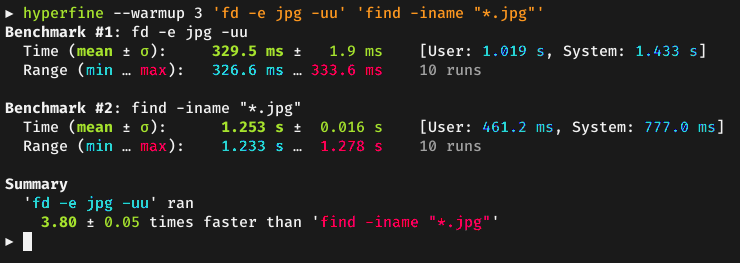
\includegraphics[width=\textwidth]{./assets/hyperfine.png}
  \caption{An example picture of Hyperfines output comparing \texttt{fd} and \texttt{find} \cite{hyperfine}}
\end{figure}

Firstly, Hyperfine supports out of the box statistical analysis and outlier detection. Since it can assume that the program run times are approximately equal, benchmark times are normal distributed. Thus, by fitting a normal distribution over all runs and computing its confidence interval, it can detect any outliers. Secondly, it allows for warmup runs and cache-clearing commands \footnote{such as \texttt{echo 1 > /proc/sys/vm/drop\_caches} to free the page cache \cite{kernel}.} between each run. Warmup runs are useful to fill caches such as the page cache for disk I/O. Lastly, it supports further analysis by providing an export to various formats, such as CSV, JSON, Markdown or AsciiDoc, which can then be analyzed programmatically. Hyperfines repository contains several python scripts for basic visualization \cite{hyperfinescripts}, which can be used as a starting point for further analysis.

\subsection{Performance Optimization}
For the benchmarking, the aforementioned \texttt{criterion.rs} benchmarking framework is used. The benchmark was done on a Dell Latitude 7420 with an Intel i5-1145G7 and 16GB of LPDDR4 RAM, compiled with rustc 1.72.0. The CPU idle was around 1\%.

\subsubsection{Call By Reference}
Although the data part of \texttt{Vec<>} is stored on the heap\footnote{Since \texttt{Vec<>} are dynamically resizable, the absolute size can't be known at compile time.} the stack-part is still very complex, since it has to keep track of several things such as the current size and its current maximal capacity. More importantly, the \texttt{Vec<>} struct has a bigger memory footprint than a pointer. Thus, using Call-By-Reference should improve the performance by requiring less memory copies! In Rust, this can be archived using the \texttt{\&} operator:

\begin{listing}[H]
  \inputminted{rust}{./assets/call_by_ref.rs}
\caption{Changing the signature to Call-By-Reference semantics with references.}
\end{listing}

Using the default criterion settings \footnote{Default Rust Release build}, the following results were benchmarked:


\begin{figure}[H]
\centering
\begin{subfigure}{.5\textwidth}
  \centering
  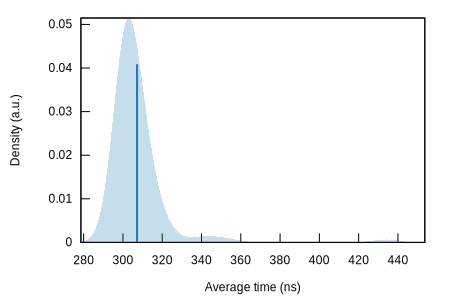
\includegraphics[width=\linewidth]{./assets/callbyvaluepdf}
  \caption{Call By Value: Mean $307.19$ns}
\end{subfigure}%
\begin{subfigure}{.5\textwidth}
  \centering
  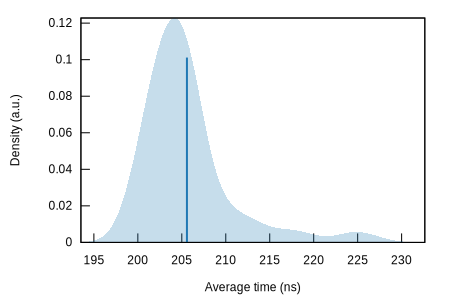
\includegraphics[width=\linewidth]{./assets/callbyrefpdf}
  \caption{Call By Reference: Mean $205.58$ns}
\end{subfigure}
  \caption{Comparsions of the \acp{PDF} computed using \ac{KDE} for Call-By-Value and Call-By-Reference.}
\end{figure}

According to the benchmarks, this change alone resulted in a $49.426\%$ mean increase! Note that the full metric table is included in the appendix.\\

There is one more obvious possible improvement to try: In this code, Rust's \texttt{Vec<>}, a dynamically sized, heap allocated vector is used. This could be replaced with a normal C-type array.

\subsubsection{Primitive Stack Arrays}
Compared to static arrays, \texttt{Vec<>} has much overhead. Firsrly, since its size is not known at compile time, it performs several run-time bounds checks \footnote{This can be partially avoided. For more information, see the bounds checks cookbook \cite{bounds_cookbook}}. Next, it has to be heap-allocated, which can be way more expensive and results in worse memory locality. Lastly, \texttt{Vec<>} is a complex struct with many functions and features, which in turn results in more computation required.\\

This is the code using primitive stack arrays instead of the more sophisticated, dynamically allocated vectors:

\begin{listing}[H]
  \inputminted{rust}{./assets/array.rs}
\caption{Changing the signature to Call-By-Reference semantics with references.}
\end{listing}

Here are the results, compared to the initial version:

\begin{figure}[H]
\centering
\begin{subfigure}{.5\textwidth}
  \centering
  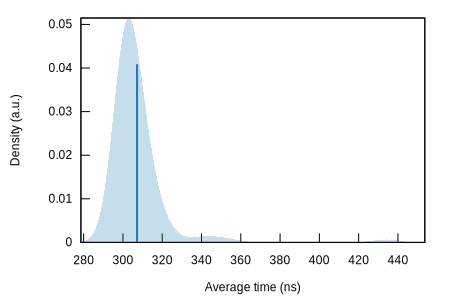
\includegraphics[width=\linewidth]{./assets/callbyvaluepdf}
  \caption{Call By Value: Mean $307.19$ns}
\end{subfigure}%
\begin{subfigure}{.5\textwidth}
  \centering
  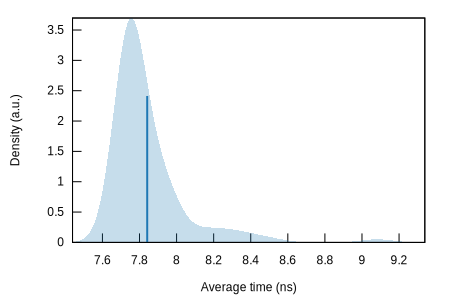
\includegraphics[width=\linewidth]{./assets/arrayspdf}
  \caption{Primitive Arrays: Mean $7.841$ns}
\end{subfigure}
  \caption{Comparsions of the \acp{PDF} computed using \ac{KDE} for the initial version and the one using primitive arrays.}
\end{figure}

This results in a staggering $3831.27\%$ mean increase! Once again, note that the full metric table is included in the appendix.\\

There are several possible explainations for those results. It could be that the bounds check ruin the instruction pipelining. But the main reason ist most likely that the prior version requires an expensive heap allocation for the return value while the static arrays are already preallocated on the stack \footnote{Further analysis could be done through statistical profiling, which will be explained later. But since it doesn't help explaining performance engineering concepts, it is left as an exercise to the reader.}. Now that we did all high-level optimizations, the next step would be to optimize on the assembly level. The next section will show how to use proper tooling for assembly level optimization in Rust.

\subsection{Assembly Optimizations}
Modern compilers, such as the \ac{LLVM} based rustc, do a lot of optimization for performance. This results in vastly different assembly when comparing unoptimized code (\texttt{-O0}) to their optimized counter part (\texttt{-O3}). Thus, it often makes sense to look at the assembly for hot code paths\footnote{Code paths are 'hot' when they are executed very frequently, therefore crucial for the overall performance.}. Naively, one could just look at the whole binary and decode the bytes into their instructions. This is neither useful nor reasonable for large programs to analyze. Instead, in this section, two different ways to analyze assembly will be analyzed: The well known Compiler Explorer \cite{compilerexplorer} as well as the \texttt{cargo-show-asm} crate \cite{cargoshowasm}.

\paragraph{Compiler Explorer}

Compiler Explorer \cite{compilerexplorer} is an online development environment initially developed by Matt Godbolt, primarily used for analysis of C and C++ applications. It was started in 2023 for optimizing financial quantitative analysis algorithms. Compiler Explorer supports over 30 different languages; from typical high performance languages such as C, C++ and Fortran, bytecode languages such as Python and Java to more niche languages such as Haskell and Solidity. Additionally, one can compare different compilers (for example \texttt{gcc}, \texttt{clang} and \texttt{msvc} for C applications) and manually specify different compiler arguments such as \texttt{-Osize} instead of \texttt{-O3}. Since it can also be hosted on-premise, propriatary and other custom compilers can be added if needed.

Its main feature is the color coding; Compiler Explorer assigns each function line to a specific color. The same color will then be used in the assembly window, providing an intuitive mapping and an good overall user experience. Unfortunately, it does not support multiple files and hasn't any dependency management \footnote{Although one could work around this restriction by installing all dependencies globally on a self hosted instance.}. To summarize, Compiler Explorer is the best fit for small, single file programs. For larger applications, the next tool can be used.

\paragraph{cargo-show-asm}

\texttt{cargo-show-asm} \cite{cargoshowasm} is a more minimalist, less polished console application for analyzing assembly. It works with any rust code base, no matter the size or amount of dependencies. Instead of showing the assembler for all functions, one can query single functions as an CLI parameter. Lastly, instead of the architecture specific assembler code it can also return the \ac{LLVM} \ac{IR} instead.

\begin{figure}[H]
\centering
\begin{subfigure}{.5\textwidth}
  \centering
  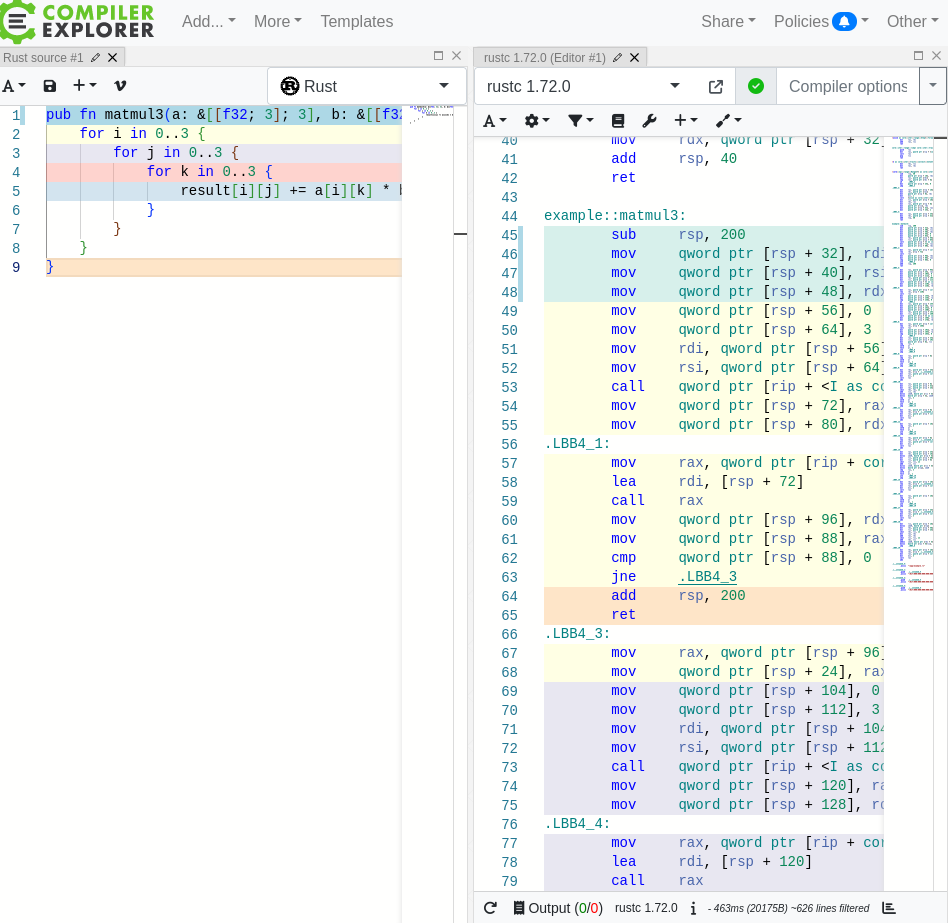
\includegraphics[width=\linewidth]{./assets/compexp}
  \caption{Compiler Explorer}
\end{subfigure}%
\begin{subfigure}{.45\textwidth}
  \centering
  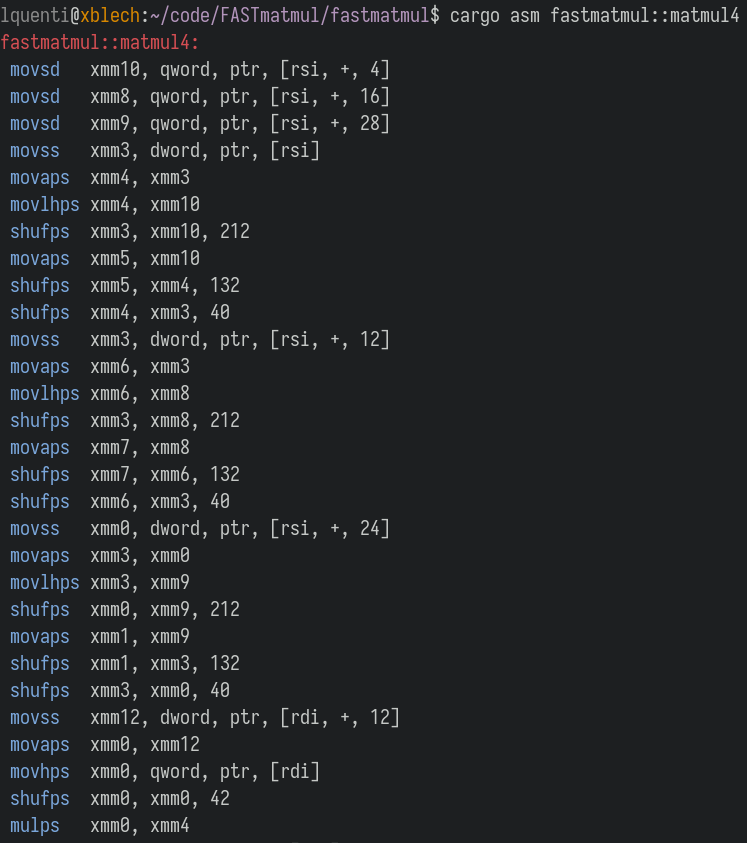
\includegraphics[width=\linewidth]{./assets/cargoasm}
  \caption{\texttt{cargo-show-asm}}
\end{subfigure}
  \caption{Two applications to analyze Rust assembly: Compiler explorer and \texttt{cargo-show-asm}.}
\end{figure}

Next, two common compiler optimizations are covered: Loop Unrolling and Function inlining.

\subsubsection{Loop Unrolling}

On the surface, loop unrolling is a simple concept: If the number of loop iterations are known at compile time, replicate the inner code that amount of time. This has multiple benefits. Firstly, it reduces the number of comparisons and jumps made in every iteration. Secondly, it allows for easier pipelining since there is no need for path prediction anymore! The main drawback is that code duplication obviously increases binary size.

Looking at the assembly, loop unrolling was already applied in our case. But if the compiler did not unroll the function, there are two main ways to force it manually:
\begin{itemize}
  \item Unroll \cite{unroll} is a Rust macro to unroll the applications at compile time by replacing the unrolled rust code in preprocessing. Currently, it can just detect loops with integer literal bounds.
  \item For more sophisticated loops, LLVM can be configured to more agressively apply loop unrolling. This is controlled by the \texttt{-unroll-threshold} parameter\footnote{So to apply it with \texttt{rustc}, use \texttt{-C llvm-args=-unroll-threshold=N} where \texttt{N} is an integer.}.
\end{itemize}
As an important remark, do not manually apply loop unrolling without benchmarking, as it can worsen performance by consuming too much of the L1 CPU instruction cache.

\subsubsection{Function Inlining}

The next, very common compiler optimization is function inlining. Instead of jumping into a subroutine, executing it, and then returning to the previous instructions it places the assembly of the subroutine into the outer function. On the upside, this eliminates the calling overhead (such as moving arguments into registers) specified by the calling convention \footnote{Interestingly, Rust does not have a default non-FFI calling convention for performance benefits. Instad, it requires all dependencies to be compiled with the same version, which is the canonical way when the package manager \texttt{cargo} is used.}. As already mentioned above, function inlining can also worsen performance though increased binary size and consequently less efficient cache utilization.

In our case, it was not applied. But it can be applied manually with the \texttt{\#[inline(/always/never)]} attribute \cite{inline}.\\

After covering benchmarking and assembly analysis, we can now approach the harder problem of variadic size matrix multiplication!

\section{Variadic Size Matrix Multplication}

Now, after having a simplified toy problem, lets say you get the following task:\\

``Our department has built a deep learning framework in Rust that inferences too slow. Please try to optimize the overall performance of this project''\\

Before being able to optimize the code, one has to first ask the following question: Why is it so slow? In order to answer this question, profiling is needed.

\subsection{Profiling}

Profiling is used to find out which parts of the program are executed frequently enough to effect runtime performance\footnote{So called \textbf{hot paths}.}. Since Rust produces normal binaries, most traditional profilers just work, including common ones such as Linux \texttt{perf} \cite{perf} and \texttt{cachegrind} \cite{cachegrind}. See the profiling section in thr Rust Performance Book for an more exhaustive list \cite{profiling}.\\

Since rust supports polymorphism\footnote{Both ad-hoc polymorphism through traits and parametric polymorphism based on generics.} name mangling occurs. As assembly labels have to be unique, name mangling is a technique used to map all polymorphic instances of a function to an unique assmbler label. If the profiler doesn't support unmangling natively, \texttt{rustfilt} can be used manually \cite{rustfilt}.\\

In this chapter, we use \texttt{cargo-flamegraph} \cite{flamegraph} and later \texttt{iai} \cite{iai} for profiling.

\subsection{Cargo Flamegraph}

Cargo flamegraph \cite{flamegraph} is a statistical profiler that creates a flamegraph to analyze. In order to understand the result, one needs to understand how statistical profilers work internally.
A statistical profiler works by interrupting the program randomly using the kernels interrupt system\footnote{Cargo flamegraph uses \texttt{perf} and \texttt{dtrace} internally.}. After interrupting, it looks at the stack frame, finding out which function stack is currently called. This is a single data point. Now, using a monte carlo approach, a statistical profiler can approximate how much time is spent in each function by taking many measurements.\\

A flamegraph is a visualization of the stack frames. The wider the current stack frame, the more often those functions were called then interrupted. One layer got called by the layer below. Here is an example of an flamegraph:

\begin{figure}[H]
  \centering
  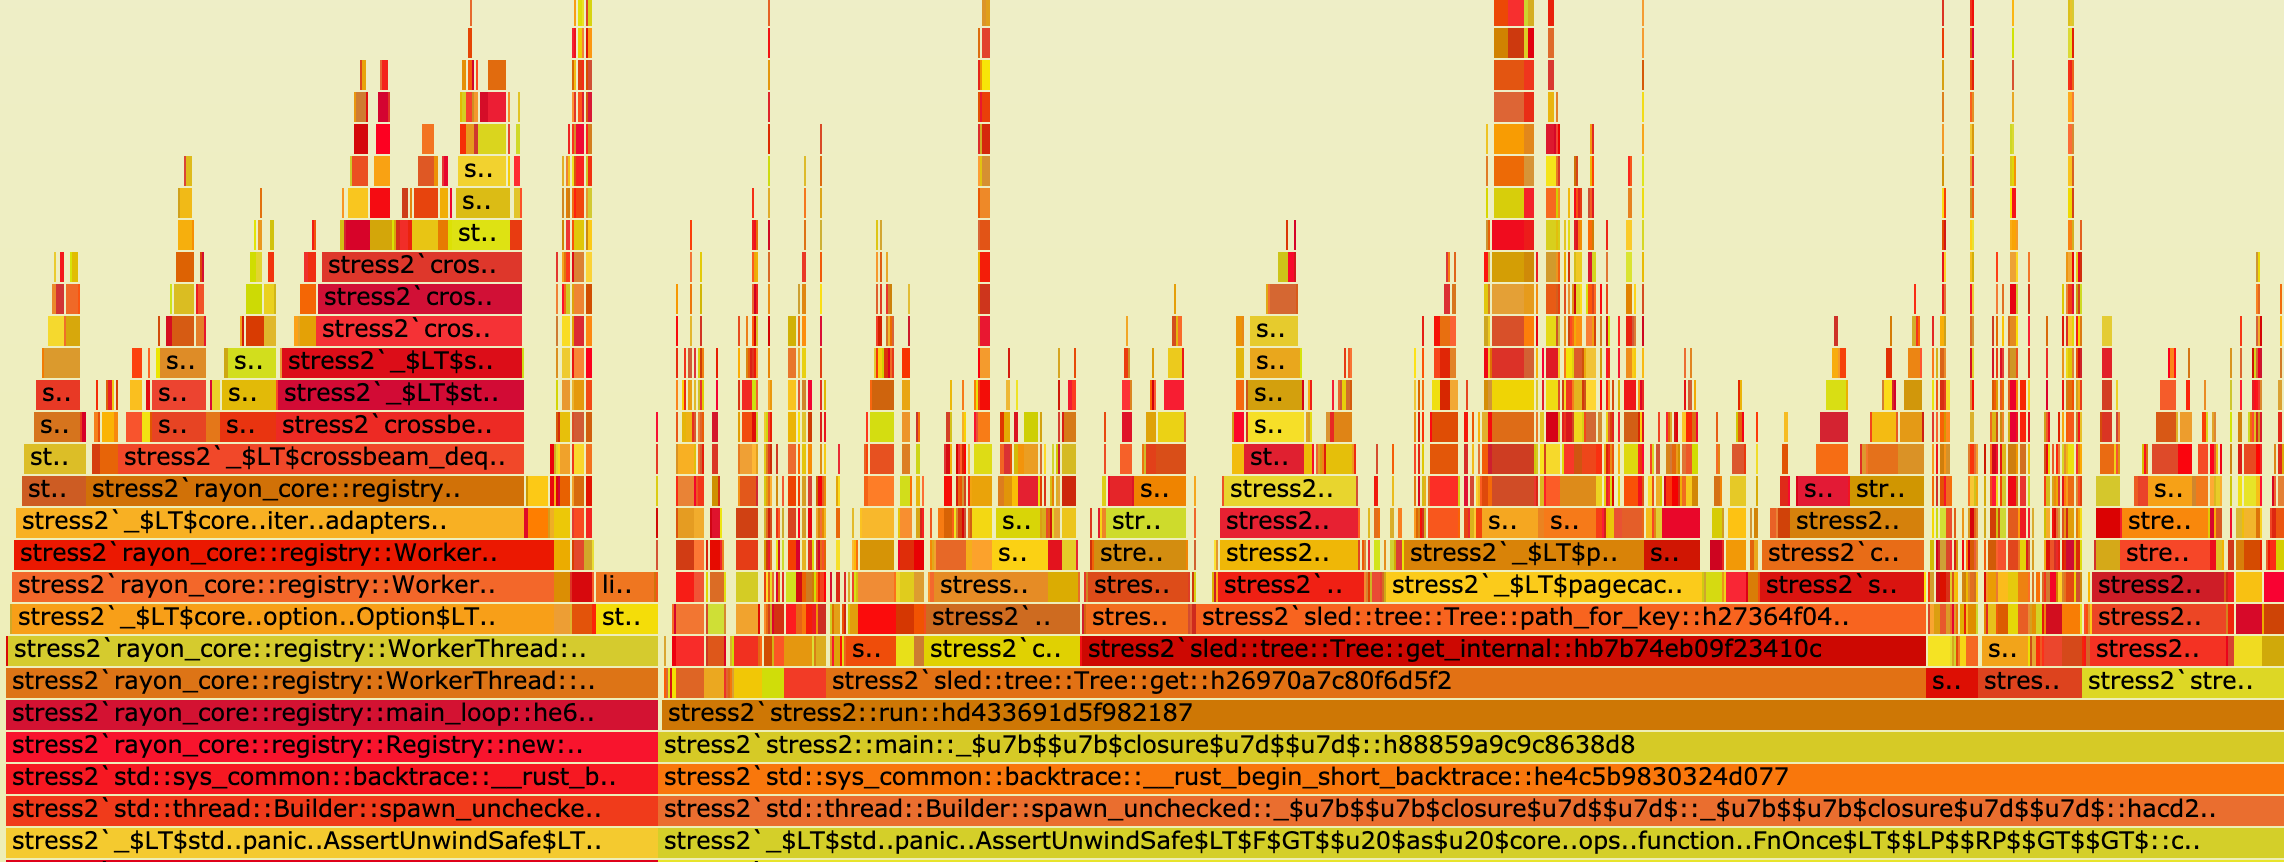
\includegraphics[width=\textwidth]{./assets/exampleflamegraph}
  \caption{An example flamegraph generated from Rust code \cite{flamegraph}.}
\end{figure}

For our fictional deep learning framework, lets assume that the result was a slow $N \times N$ variadic size matrix multiplication! For the benchmarks, we use $N=1024$.

\subsection{Applying Previous Knowledge}
Lets say that the matrix multiplication function looks as follows:

\begin{listing}[H]
  \inputminted{rust}{./assets/variadic_unoptimized.rs}
\caption{The unoptimized Rust code providing the variadic size quadratic matrix multiplication}
\end{listing}

Applying the knowledge of our previous chapters, we can already refactor it into the following:

\begin{listing}[H]
  \inputminted{rust}{./assets/variadic_optimized.rs}
\caption{The code optimized analagously to chapter 2.}
\end{listing}

But before benchmarking this code, there are further free improvements to be had by configuring the compiler to maximize performance.

\subsection{Compiler Optimizations}
There are several performance optimizations that should be enabled if performance is a high priority:
\begin{itemize}
  \item \textbf{Release Builds}: This is by far the biggest improvement. If one does not use the release build\footnote{With \texttt{cargo build --release}.} the code is not optimized. This enables several general optimizations as well as automatic vectorization.
  \item \textbf{\ac{LLVM} \ac{LTO}}: \ac{LTO} enabled further, intermodular optimizations during the link stage. While this could improve code by optimizing beyond library bounds, it increases compile time, which is why it is disabled by default.
  \item \textbf{Compiling for Native Architecture:} When compiling for the native architecture\footnote{Using the \texttt{RUSTFLAGS} environment variable, i.e. \texttt{RUSTFLAGS="-C target-cpu=native" cargo build --release}.} the compiler can use more specialized instructions that are not available on every processor such as bigger vector registers for SIMD. Note that this makes the code incompatible with older processor generations.
  \item \textbf{Using a single \ac{LLVM} codegen unit:} Codegen units are analagous to translation units. This means that, when changing a single file, just the codegen unit in that file has to be recompiled. Therefore, optimizations can't be done beyond codegen unit bounds! Using a single codegen for the whole project allows the compiler to more agressively optimize globally. Note that this effectively disables partial compilations.
  \item \textbf{\ac{PGO}:} \ac{PGO} could furthermore be used for more effective branch prediction\footnote{This is out of the scope for this project, for an introduction see how the compiler team used it on \texttt{rustc} \cite{pgo}}.
\end{itemize}

Here are the results, the full table can be found in the appendix:

\begin{figure}[H]
\centering
\begin{subfigure}{.33\textwidth}
  \centering
  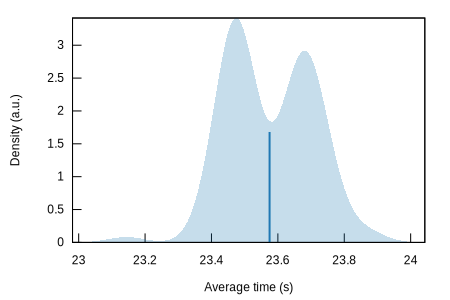
\includegraphics[width=\linewidth]{./assets/nocompiler_unoptimized}
  % hacky but works
  \caption{No compiler optimizations.\\\hspace*{0.6cm}Naive code.\\\hspace*{0.6cm}Mean: $23.575$s}
\end{subfigure}%
\begin{subfigure}{.33\textwidth}
  \centering
  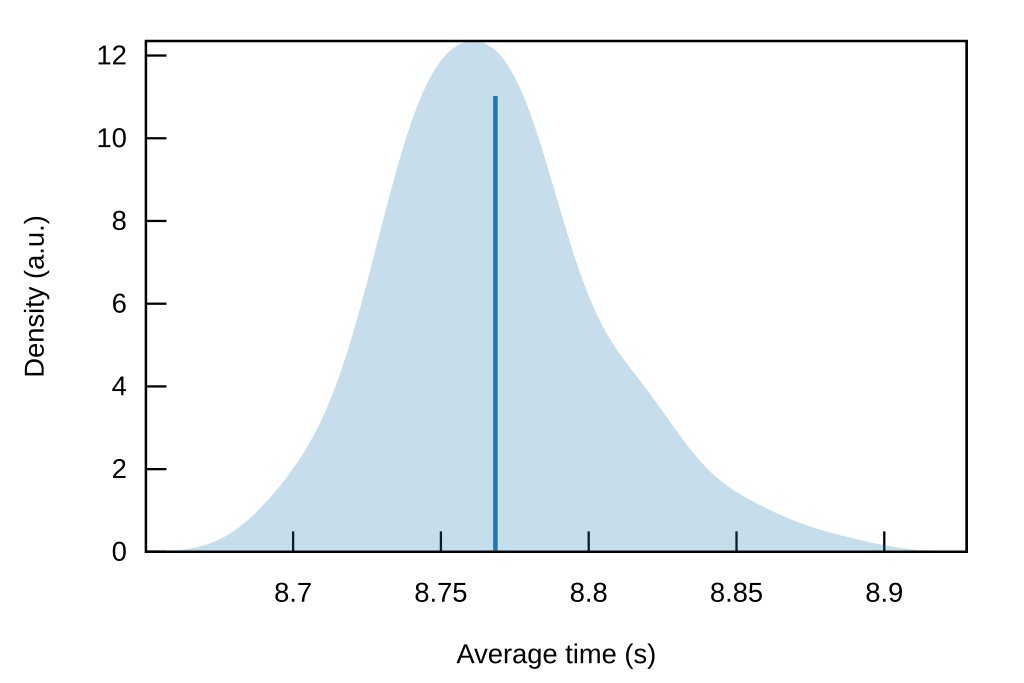
\includegraphics[width=\linewidth]{./assets/nocompiler_optimized.png}
  \caption{No compiler optimizations.\\\hspace*{0.6cm}Optimized code.\\\hspace*{0.6cm}Mean: $8.7684$s}
\end{subfigure}%
\begin{subfigure}{.33\textwidth}
  \centering
  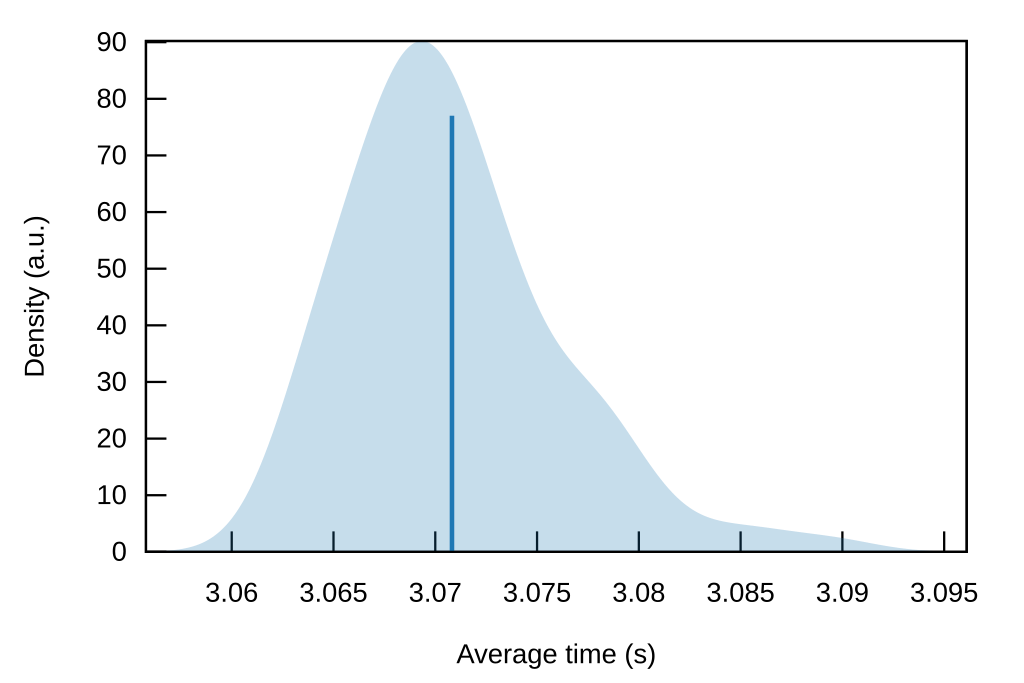
\includegraphics[width=\linewidth]{./assets/compiler_optimized.png}
  \caption{Compiler optimizations.\\\hspace*{0.6cm}Optimized code.\\\hspace*{0.6cm}Mean: $3.0708$s}
\end{subfigure}%
  \caption{Performance comparison between unoptimized code, optimized code and optimized code with compiler optimization enabled.}
\end{figure}

For the next and last optimization, some further theory is needed.
\subsection{Cache-oblivious Algorithms}

When doing a standard matrix multiplication $C:=A \cdot B$, $A$ traverses the matrix in row-major order and $B$ traverses the matrix in column-major order. Since the memory is aligned in row-major order, in every step of $B$ we get a cache miss for large sizes of $B$.

\begin{figure}[H]
  \centering
  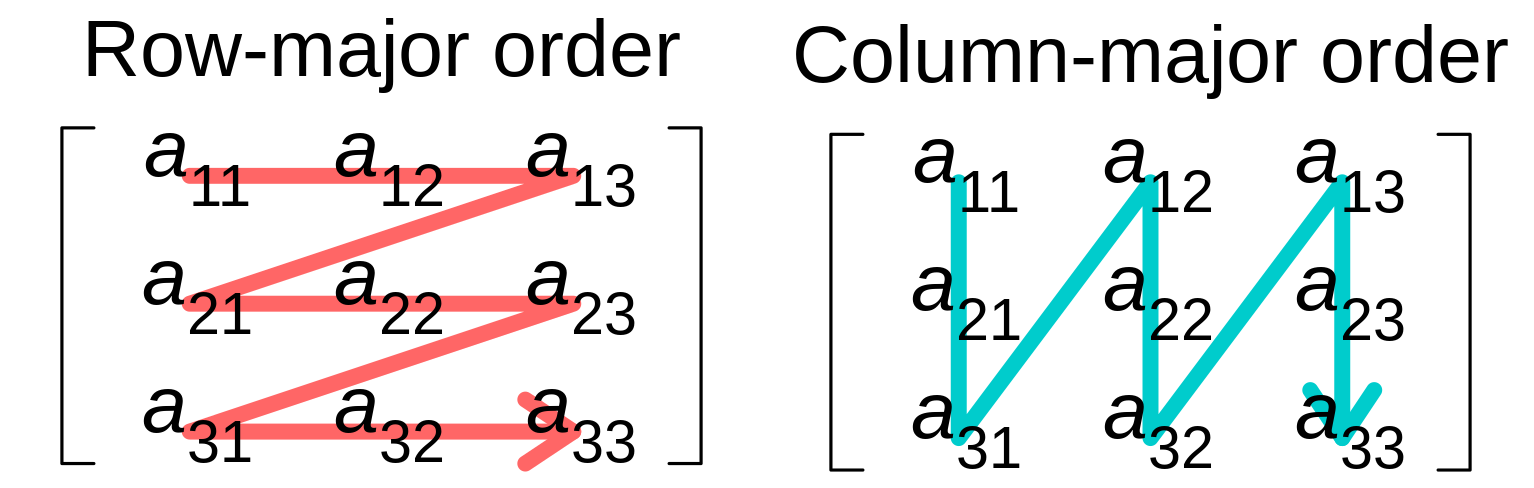
\includegraphics[width=0.8\textwidth]{./assets/rowcol}
  \caption{A visualization of row- and column-major order.}
\end{figure}

A possible solution could be to compute $A \cdot B^T$ instead by transposing $B$. Then, $C_{ij}$ is computed as row $A_i$ times \textbf{row} $B_j$! Unfortunately, since we have to actually compute the transpose beforehand, this requires $\Theta(n^2)$ precompute.

Naturally, two questions arise:
\begin{enumerate}
  \item Does it improve speed?
  \item Does it actually reduce cache misses?
\end{enumerate}

Whether it improves speed can easily be benchmarked.

\begin{figure}[H]
\centering
\begin{subfigure}{.5\textwidth}
  \centering
  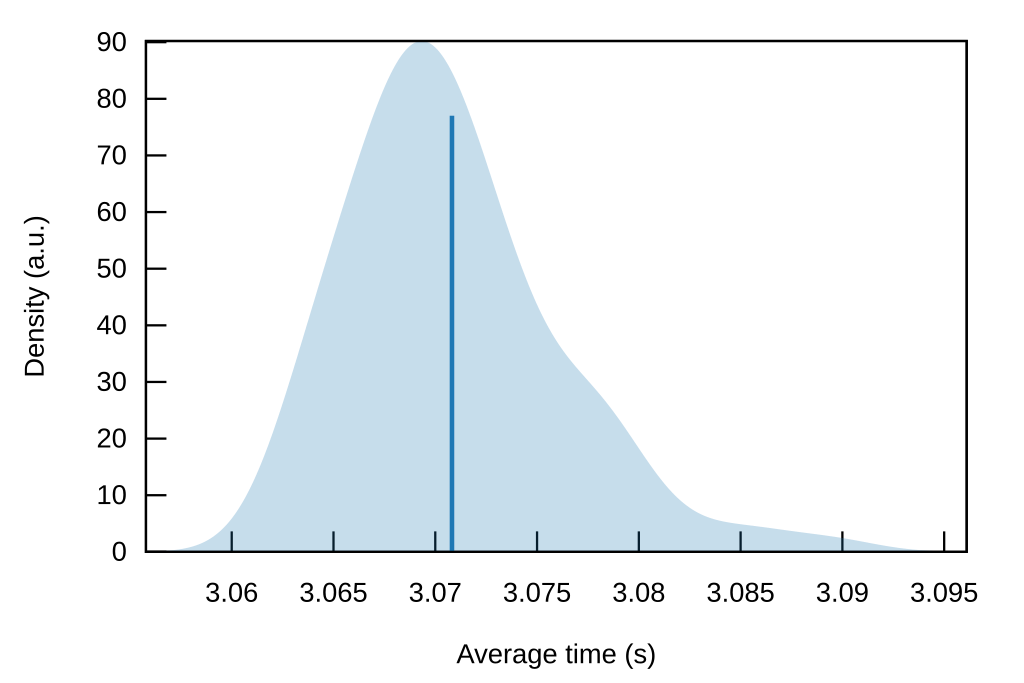
\includegraphics[width=\linewidth]{./assets/compiler_optimized.png}
  \caption{Compiler optimizations.\\\hspace*{0.6cm}Optimized code.\\\hspace*{0.6cm}Mean: $3.0708$s}
\end{subfigure}%
\begin{subfigure}{.5\textwidth}
  \centering
  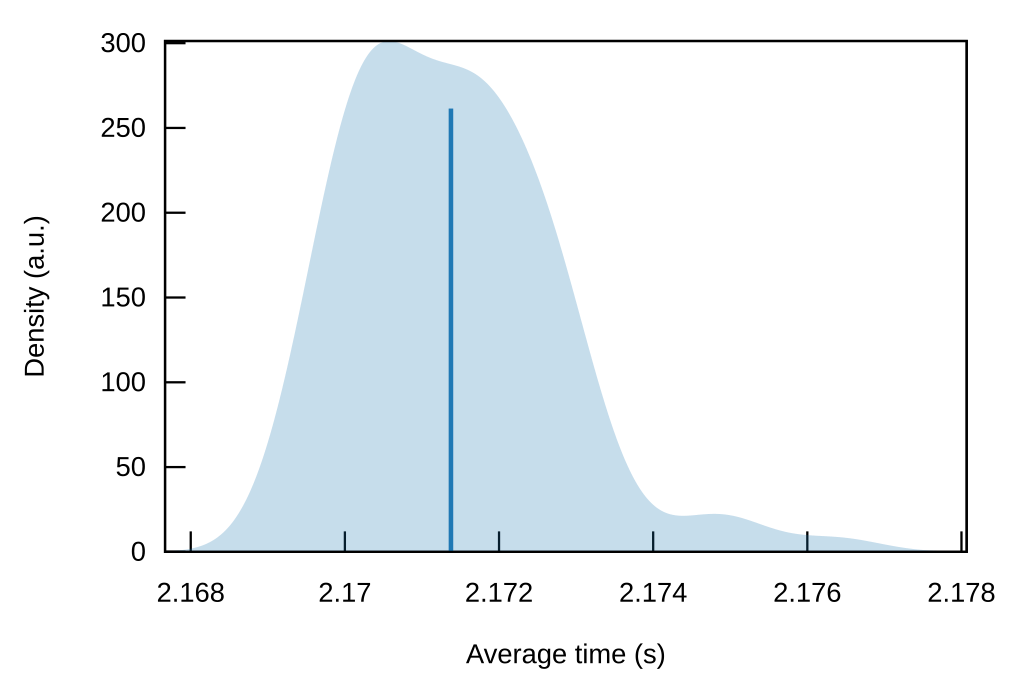
\includegraphics[width=\linewidth]{./assets/compiler_optimized_transposed.png}
  \caption{Compiler optimizations.\\\hspace*{0.6cm}Optimized and transposed code.\\\hspace*{0.6cm}Mean: $2.1714$s}
\end{subfigure}%
  \caption{Performance comparison between unoptimized code, optimized code and optimized code with compiler optimization enabled.}
\end{figure}

For finding out whether it reduces cache misses, we can use \texttt{iai}.

\subsection{Iai}
\texttt{Iai} \cite{iai} is a high-precision, one-shot benchmark framework for Rust code. One-shot means that the code is only run a single time. This is possible by leveraging cachegrind \cite{cachegrind} under the hood to simulate the CPU and its caches, allowing us to count all cache accesses. Furthermore, it can be used for \ac{CI} pipelines since it solves the noisy-neighbour problem of multiple jobs executed on the same runner. Here are the results:

\begin{listing}[H]
  \inputminted{text}{./assets/iai.txt}
\caption{The results running iai}
\end{listing}

Here one can see that, although more RAM accesses, it has better L1 and L2 utilization.

\section{A glimpse of (Inter-Node) Parallelism}
Rust has many ways to do inter-node parallelism\footnote{Rust also support intra-node parallelism using \texttt{rsmpi} \cite{rsmpi}, a rust-native MPI library compatible with OpenMPI and MPICH. Unfortunately, this is out of scope here. For more information, see my report on walky \cite{walky}, the rusty TSP solver.}. One can categorize iner-node parallelism into two categories: Single thread parallelism using SIMD instructions and multi threading. In this chapter, we will give a high-level overview how to archive both.

\subsection{SIMD}
While a complete introduction in \ac{SIMD} programming would be an report on its own\footnote{For a great introduction on how to do \ac{SIMD} in Rust, see the \ac{SIMD} Rust on Android Talk by Guillaume Endignoux \cite{simdtalk}.} it is noteworthy to say that Rust has two different approaches to support \ac{SIMD} programming. The old, processor specific API and the new, portable SIMD API.

\paragraph{Processor specific API:} The processor specific API is experimental only and classified as unsafe, i.e. it doesn't give any memory guarantees. It is composed of the direct low level intrinsics procided by the CPU manufacturer and has the same function definitions as the C API. The only reason is that it is part of the \texttt{core} instead of \texttt{std} library: This means, it does not expect any memory allocator nor any OS syscalls to work properly and can thus we used bare metal.

\paragraph{Portable SIMD:} The portable \ac{SIMD} API is, while also experimental, memory safe. Instead of providing instructions for any CPU architecture, it is generalized on a bit level with types such as \texttt{std::simd::\{f32x8, f64x4, i32x8\}}. This makes it the preferred API for non-bare metal programming. It is part of the \texttt{std} library.\\

Lastly, note that code that does not have those processor features will produce undefined behaviour. There are two ways to mitigate this: If the target architecture is known at compile time, Rust supports conditional compilation\footnote{Compile for specific architecture: \texttt{\#[cfg(target\_arch="x86\_64")]}}\footnote{Compile for specific feature: \texttt{\#[cfg(target\_feature="aes")]}} to provide alternatives to architecture specific code. If this is not the case, functions such as \texttt{std::is\_x86\_feature\_detected} can be used. Note that these should not be used in hot loops as they provide an runtime overhead.

\subsection{Multithreading}

Rust supports several ways of doing multi threading. First of all, the standard library offers many primitives around simple OS-threads\footnote{Rust also supported green threads before 1.0 but they were cut because the scheduling menat that they were not zero cost.} See the ``Fearless Concurrency'' chapter of the Rust book for an introduction \cite{conbook}.\\

Furthermore, Rust provides an \texttt{async/await} pattern for managing async \ac{I/O}. In order to enable the usage in many, vastly different environments such as \ac{IoT}, Rust requires the developer to bring their own async runtime. Most projects use \texttt{Tokio} \cite{tokio}, although other projects such as the simpler \texttt{smol} or \texttt{fuchsia-async} \cite{fuchsia} used in Googles Fuchsia. For more information to \texttt{async/await}, see the official async book \cite{asyncbook}, the announcement talk from WithoutBoats \cite{withoutboats} or fasterthanlimes ``Understanding Rust futures by going way too deep'' \cite{fasterthanlime}.\\

Lastly, there are several utility libraries. Here, we will focus on \texttt{rayon} because of its simplicity.

\subsubsection{Rayon}

Rayon is a high-level parallelism library using dynamically sized thread pools. It guarantees \textbf{data-race freedom} by allowing only one thread to write at a time. Its main features are drop-in parallel iteratiors: By replacing \texttt{.iter()} with \texttt{.par\_iter}, it is possible to use all functions provided for iterators, such as \texttt{.map()}, \texttt{.filter()}, \texttt{.reduce()} for typical functional patterns or \texttt{.join(|| a(), || b()} enabling the \texttt{fork-join} computation model.
It is best explained with a code example. Lets rewrite our function in a more iterator based version:

\begin{listing}[H]
  \inputminted{rust}{./assets/02rayon.rs}
\caption{An more functional version of our matrix multiplication}
\end{listing}

This can be parallelized by only replacing \texttt{.iter\_mut()} with \texttt{.par\_iter\_mut()}:

\begin{listing}[H]
  \inputminted{rust}{./assets/03rayon.rs}
\caption{This is the parallelized version, changing a single function call!}
\end{listing}

\section{Conclusion and Further Ressources}

To conclude, although many parts are still experimental, all tooling for proper performance engineering exists, making Rust a viable programming language for \ac{HPC}. A summary of all tools can be found in the appendix.\\

If one is more interested in performance engineering, the best resources for understanding performance tuning in Rust is the ``Rust Performance Book'' \cite{rperfbook}. To understand more about performance engineering and the theory behind it, the free online book ``Algorithmica: Algorithms for Modern Handware'' \cite{algomodern} is a good starting point. Finally, if one is more interested in intra-node parallelism, the \texttt{rsmpi} library \cite{rsmpi} has great examples to get started.

% TODO TABELLE IN APPENDIX
